\FloatBarrier

Using the same circuit as before, i_{D}$ was measured while sweeping $V_{DS}$ for $V_{GS}$ = 2.5$\si{\volt}} and then 5.0$\si{\volt}} and keeping $V_{SB}$ = 0$\si{\volt}}.
Results are shown in Figure 2a and 2b.

\begin{figure}[h!]
	\centering
	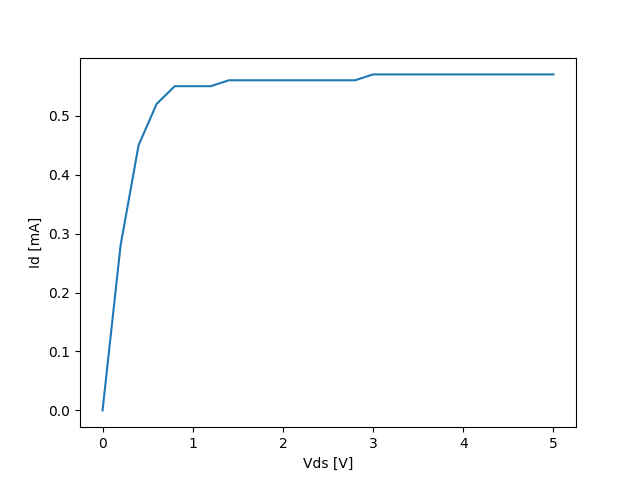
\includegraphics[scale=0.75]{../images/data_2.PNG}
	\caption{$i_{D}$ versus $V_{DS}$ of NMOS where $V_{GS}= 2.5$\si{\volt}}
	\label{fig:data_3}
\end{figure}
\FloatBarrier

\FloatBarrier

\begin{table}[h!]
	\centering
	\caption{Figure (\ref{fig:data_2}) Data}
	\label{tab:data_2}
	\csvautotabular{../tables/data_2.csv}
\end{table}

\FloatBarrier

\begin{figure}[h!]
	\centering
	\includegraphics[scale=0.75]{../images/data_2b.PNG}
	\caption{$i_{D}$ versus $V_{DS}$ of NMOS where $V_{GS}= 5$\si{\volt}}
	\label{fig:data_2b}
\end{figure}
\FloatBarrier

\FloatBarrier

\begin{table}[h!]
	\centering
	\caption{Figure (\ref{fig:data_2b}) Data}
	\label{tab:data_2b}
	\csvautotabular{../tables/data_2b.csv}
\end{table}

In both cases of $V_{GS}$, the transistor saturates near the value of $V_{GS}$ - $V_{t}$.
For $V_{GS}$ = 2.5$\si{\volt}}, this value is about 0.8$\si{\volt}}, and for $V_{GS}$ = 5.0$\si{\volt}}, saturation occurs at around 3$\si{\volt}}
This suggests that $V_{t}$ is around 1.8$\si{\volt}}, consistent with what was found in part 1.
